%\documentclass[11pt,a4paper]{jreport}                    % fir platex
\documentclass[11pt,a4paper,uplatex]{ujreport} 	% for uplatex
%
\usepackage{amsmath,amssymb}
\usepackage{bm}
\usepackage{graphicx}
\usepackage{ascmac}
\usepackage{float}
%
\setlength{\textheight}{40\baselineskip}
\addtolength{\textheight}{\topskip}
\setlength{\voffset}{-0.2in}
\setlength{\topmargin}{0pt}
\setlength{\headheight}{0pt}
\setlength{\headsep}{0pt}

\setlength{\textwidth}{\paperwidth}     % ひとまず紙面を本文領域に
\setlength{\oddsidemargin}{-5.4truemm}  % 左の余白を20mm(=1inch-5.4mm)に
\setlength{\evensidemargin}{-5.4truemm} % 
\addtolength{\textwidth}{-40truemm}     % 右の余白も20mmに
%
\newcommand{\divergence}{\mathrm{div}\,}  %ダイバージェンス
\newcommand{\grad}{\mathrm{grad}\,}  %グラディエント
\newcommand{\rot}{\mathrm{rot}\,}  %ローテーション
%
\title{脳を学ぶ上で重要な数学シリーズ 応用編}
\author{後藤 優仁}
\date{\today}
\begin{document}
\maketitle
%
%
\tableofcontents


\chapter{信号処理}

さて, 基礎を学んだところで, ここからはいよいよ理工系の学生, 脳というブラックボックスに挑む学生として学ぶべき, 高度な数学に挑戦していきます.\\ 
わくわくしますね!!!\\
\section{オイラーの公式 \label{euler}}
まずはオイラーの公式の導出からいきましょう!!!\\
\\
今まで, 証明をずっと後回しにしてたくせによく使っていた理由は, まずこの公式の導出には様々な数学的知識が必要であることです. また, やや直感的に分かりにくい公式であるため, 導出より先にその利便性, 利用のされかたに触れて慣れてほしかったのです.\\

\subsection{オイラーの公式を翻訳する}
改めて, オイラーの公式を眺めてみましょう.\\
\begin{eqnarray}
\mathrm{e}^{i\theta} = \cos\theta + i\sin\theta
\end{eqnarray}
うーん, 美しいですね.\\
\\
こいつをちょっと解剖してみましょう. 数学語を日本語に翻訳すると, おそらくこんな感じになります.
\\
\\
底をネイピア数eとし, 指数関数 $\mathrm{e}^x$のxに角度Θを代入し, 虚数単位iをかけたもの(左辺)が, sin と cos の足し算で表した何らかの値と同じ値を表している.\\
\\
うーん謎ですね.\\
なぜ指数関数が三角関数で表せるのか?\\
三角関数の足し合わせってなんだよ?\\
指数関数を虚数にするってなんだよ??\\
\\
\\
私はここで脳がオーバーヒートを起こし, 拒絶反応を起こしたものです.\\
\\
\\
どうしても分からないのは無視しよう!!!\\
\\
というのも, オイラーの公式は偶然発見されたと考えた方が気が楽になるのです. 厳密に理解するのは難しい.\\
\\
\\
理解が進めば, おのずと脳に適用されます.
\subsection{マクローリン展開}
さて, 一旦オイラーの公式は忘れてみましょう.\\
\\
大学で学ぶ数学, とりわけ微分積分において最初に我々が躓く単元に, テイラー展開・マクローリン展開がありますね!\\
\\
オイラーの公式は, このマクローリン展開さえ分かれば一瞬で導出する事が可能です.\\
\\
はじめに,テイラー展開とマクローリン展開の違いは, テイラー展開の限定された特殊形がマクローリン展開です. なのでマクローリン展開だけここでは扱います.\\
\begin{eqnarray}
f(x) = \sum_{k=0}^\infty f^{(k)} (0) \frac{x^k}{k!} = f(0) + f'(0)x + \frac{f''(0)}{2!}x^2 + \frac{f'''(0)}{3!}x^3 ...
\end{eqnarray}

これがマクローリン展開です.\\
元関数f(x)を多項式で近似するわけですね.\\
\\
ここで使われる多項式は, 元関数fのx=0の時の高階微分係数から定まっています.\\
\\
こいつの凄いのは, 局所的なある一点での振る舞いだけをみれば元の関数がわかるって事です!!\\
テイラー展開とは, この時のxの値が0じゃなくてどこでもいいってやつで, マクローリン展開はx=0に限ったやつの事です.\\
\\
x=0の時に最も元関数っぽい一次関数, 二次関数, 三次関数...と∞に足し合わす事で元関数を表そうって事です!!!\\
便利そうですね. 計算はだるいが.\\
\subsection{指数関数と三角関数のマクローリン展開}
さて, ここで指数関数と三角関数(sin, cos)のマクローリン展開を見てみましょう!!\\

\begin{figure}[H]
\label{im:exp}
  \centering
  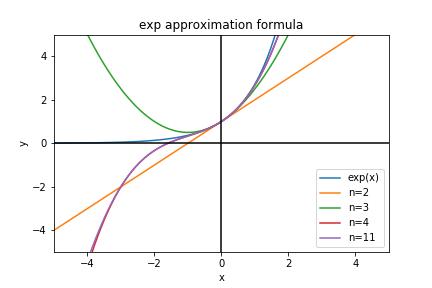
\includegraphics[width=120mm,bb=0 0 432 288]{figures/exp.png}
  \caption{exp関数のマクローリン展開}
\end{figure}
\begin{figure}[H]
\label{im:sine}
  \centering
  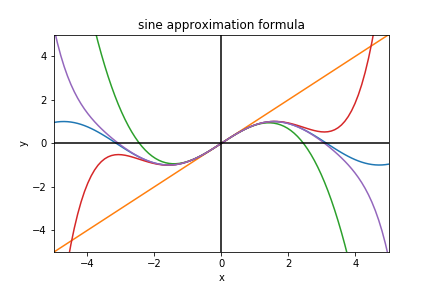
\includegraphics[width=120mm,bb=0 0 432 288]{figures/sine.png}
  \caption{sin関数のマクローリン展開}
\end{figure}

\begin{figure}[H]
\label{im:cosine}
  \centering
  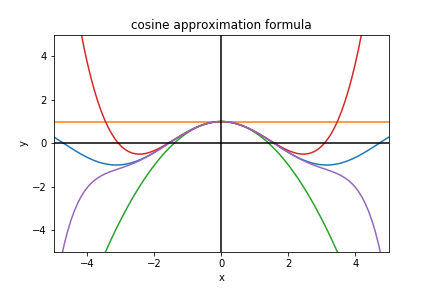
\includegraphics[width=120mm,bb=0 0 432 288]{figures/cosine.png}
  \caption{cos関数のマクローリン展開}
\end{figure}

\begin{eqnarray}
\mathrm{e}^x = \sum_{(k=0)}^\infty \frac{x^k}{x!} = 1 + \frac{x}{1!} + \frac{x^2}{2!} + \frac{x^3}{3!} + ...
\label{eq:sisuu}
\end{eqnarray}

\begin{eqnarray}
\sin x = \sum_{k=0}^{\infty}(-1)^k \frac{x^{2k + 1}}{(2k + 1)!} = \frac{x}{1!} - \frac{x^3}{3!} + \frac{x^5}{5!} - \frac{x^7}{7!} +  ...
\label{eq:sain}
\end{eqnarray}

\begin{eqnarray}
\cos x = \sum_{k=0}^\infty(-1)^k \frac{x^{2k}}{(2k)!} = 1 - \frac{x^2}{2!} + \frac{x^4}{4!} - \frac{x^6}{6!} + ...
\label{eq:cosa}
\end{eqnarray}

賢い人なら気付くかもしれません!!!\\
気付きますよね??\\
気付かないわけがありません.\\
なんとなくですが, 式(\ref{eq:sain})と式(\ref{eq:cosa})を足すと, 式(\ref{eq:sisuu})っぽいですよね!!\\
\\
え?違うじゃんって?\\
うるせえよ, だいたい一緒だろうが.\\
\\
\\
細かいやつは女の子に嫌われるんだぞ!この陰キャが!!\\
\\
陽キャの僕はとりあえず足してみます.
\\
\begin{eqnarray}
\mathrm{e}^x = \sum_{(k=0)}^\infty \frac{x^k}{x!} = 1 + \frac{x}{1!} + \frac{x^2}{2!} + \frac{x^3}{3!} + \frac{x^4}{4!} + ...
\end{eqnarray}
\begin{eqnarray}
\sin x + \cos x = 1 + \frac{x}{1!} - \frac{x^2}{2!} - \frac{x^3}{3!} + \frac{x^4}{4!} + ...
\label{eq:mix}
\end{eqnarray}

うーん, 惜しいですよね. もうちょっと, あとは符号だけ変えちゃえば大丈夫そうなのですが...\\
2項ずつ, 符号があってたりあってなかったりしてますね.\\
\\
これは一寸難しいですね. もし交互に異なるのであれば, 式(\ref{eq:mix})の構成要素のどちらかに -1 をかければ良いのですが, 2項ずつとなるとそうもいきません. かといって両方にマイナスをかけても, 違う形になるし...\\
\\
この段階で, 操作するべきは指数関数と, 三角関数のどちらかという指針がたちます.\\
\\
しかし, そのまま-1をかけても意味がない. そこで式に注目すると, 何乗もしています. なんとか乗した時に符号が変わればいいのですから, ここで虚数単位iの導入に目星をつけます.\\
\\
とりあえず指数の方にやってみましょう.
\begin{eqnarray}
\begin{split}
\mathrm{e}^{ix} \\
& = \sum_{(k=0)}^\infty \frac{ix^k}{x!} = 1 + \frac{ix}{1!} + \frac{i^2x^2}{2!} + \frac{i^3x^3}{3!} + \frac{i^4x^4}{4!} + ...\\
& = 1 + i\frac{x}{1!} - \frac{x^2}{2!} - \frac{ix^3}{3!} + \frac{x^4}{4!} + ...
\label{eq:eix}
\end{split}
\end{eqnarray}
ちょっといい感じですね.\\
次に, 分母が奇数の時にiが残ってしまっているので, 奇数に対応しているsinの方にもiをかけてみましょう!\\
\begin{eqnarray}
i\sin x = \sum_{k=0}^{\infty}(-1)^k \frac{ix^{2k + 1}}{(2k + 1)!} = \frac{ix}{1!} - \frac{ix^3}{3!} + \frac{ix^5}{5!} - \frac{ix^7}{7!} +  ...
\end{eqnarray}
問題なさそうですね!改めてcosと足してみます!!\\
\begin{eqnarray}
\cos x + i\sin x = 1 + i\frac{x}{1!} - \frac{x^2}{2!} - \frac{ix^3}{3!} + \frac{x^4}{4!} + ...
\label{eq:cossin}
\end{eqnarray}
式(\ref{eq:eix})と式(\ref{eq:cossin})を見比べると, 見事に一致しています!!!\\
\\
これでオイラーの公式の証明がおわりですね!!\\
\\
オイラーの公式とは, 指数関数と三角関数をマクローリン展開した際にでてきた奴らが似ていたので, 虚数を導入してみたらきれいに等号で結べたねって事です.\\

\subsection{オイラーの公式の有用性}
オイラーの公式とは
\begin{eqnarray}
\mathrm{e}^{i\theta} = \cos \theta + i\sin \theta
\end{eqnarray}
であった.\\
\\
この時, Θにπを代入すると, 更に美しくなります.
\\
\begin{eqnarray}
\mathrm{e}^{i\pi} = -1 + 0\\
\mathrm{e}^{i\pi} + 1 = 0
\end{eqnarray}
実際に計算すれば分かりますね. たしかに成り立ちます. \\
最も基本である数字0と1, そしてネイピア数, 円周率, 虚数...\\
数学において偉大と言われる奴らが一堂に会して, あっさりとまとまっているのです!!!\\
ひええええ...!!!\\
\\
これこそが, オイラーの公式が人類の至宝といわれる所以ですね!\\
\\
\\
さて, オイラーの公式を信号処理の数学にどのように使っていくかというと, ざっくりした流れはこうだ!!!\\
\begin{itemize}
 \item 取得した関数を三角関数の和で表す
 \item 複素平面にもってきて極座標で表す
 \item 極座標を指数関数に変換する
 \item 計算がめっちゃ楽だし, 多次元のデータを取得できる
 \item 色々わかる!!うれしい!!
\end{itemize}
厳密に言うと脳波は定常性をもっていないので三角関数の和で表す事は出来ないんだが, 短時間の窓を設けたりウェーブレットを使う事によってそこは解決できる. \\
とりあえず今は, オイラーの公式を使う事によって脳波を簡単な形で表せる上にいろんな情報を読み取れるようになる!!すごい!!偉大だ!!!\\
\\
だけ分かればいい.\\
次節から実際にフーリエ変換などで使っていくので, オイラーの公式は脳にフィットさせといてください.\\

崇めよ!!!!!\\

\section{フーリエ変換}
さて, いよいよ本節から実際に我々が脳波と戦う際に用いる技の紹介となっていきます. 前章(\ref{basics})が理解できている諸君なら, それほどつまずく事もないはずです. 実際僕は, 前章に値する内容の理解と精査に非常に時間をかけましたが, これ以降はそれほど時間をかけずに理解を進める事が出来ました. 基本を忘れず臨んでください.
\subsection{脳波とは}
そもそも, 解析方法を考える以前に...\\
我々は脳波という似非科学チックな香ばしいものと対峙するわけですが, こいつの特性を知らずに武器や魔法を準備するのは非効率ですね. まずは脳波というものがどういったものなのかを考えてみます. \\
\\
脳波とは, 脳に無数に存在する脳神経細胞が刺激を受け, その総量が閾値を超えた時に発生される電気信号 ... の集合体の事です.\\
\\
領域Aに脳細胞が100万個あったとしましょう. \\
そのうち, 70万個が発火していて, 30万個が沈黙していたとします. 領域A直上にある脳波計の電極は, そこら一帯の電気的活動の総和を観測し, 領域Aで強い活動があったと記すわけです(図\ref{im:topo}).\\
\\
この時の「強い活動」というのは, 電極で計測された電気信号の振幅, 100万の細胞電位の総和の値です. これが大きい程, 強い活動という解釈がされます.\\

\begin{figure}[H]
\label{im:topo}
  \centering
  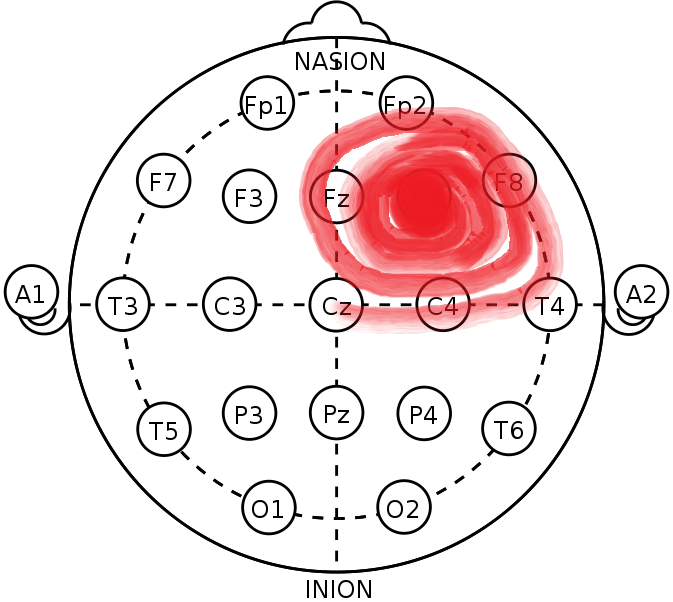
\includegraphics[width=120mm,bb=0 0 673 602]{figures/topomap.png}
  \caption{電極で拾われる脳波のイメージ. 近傍電位の総和}
\end{figure}

しかし, 元来神経細胞の1回の発火は一瞬のものです. 2つの細胞があったとして, それらが数ms間隔で交互に活動しているとしたら, 片方が発火している間にもう片方は負の方向に電位を発しているわけですから, その総和を取ると細胞1個の発火分にも満たない事になります. \\
これは当然, 数百万単位の細胞が集まった時にも同じ事が言えて, 振幅が小さいからといって脳が活動していない ... という訳ではありません. 単に同期的活動を行っているわけではないという事です.\\
\\
本来はパルス波っぽい挙動をする神経信号ですが, それらが無数に存在し, 各々のタイミングで活動をしているため, 脳波計の電極によって計測される信号は連続的で, 非常に複雑な挙動を取る波となります. \\
\\
この波を俗に脳波と言い, 振幅が大きい時には強い活動 (正確には同期した活動) が行われていて, 逆に振幅が小さい時には同期していない, つまり適当な活動を行っているといった解釈がなされたりします. \\
しかしこのままでは, 複雑すぎて人間の目で見たら何がどうなっているのか全く分からず, 麻酔科医やてんかんの診断をする超能力医者のようなスーパーマンでもない限り, 「これは○○の脳波だ!」とか言えません. そこで凡人の我々は, どうにかしてこの複雑怪奇な脳波を解釈し, 脳の活動を解明する必要があるわけです.\\

そこで, 最も基礎となるアプローチが...\\
複雑すぎて分からないなら, 単純な波に分解してあげればいいじゃん??\\ 
というやつです. どんな波も, 直交性をもつ波に分解できるみたいな話題が前章にありましたよね?あれを利用します!!
\\
こうして, 複雑極まりない脳波を, 単純で解釈のしやすい三角関数の足し合わせとして表現しよう!というのがフーリエ変換のモチベーションです.\\

\begin{figure}[H]
\label{im:eeg}
  \centering
  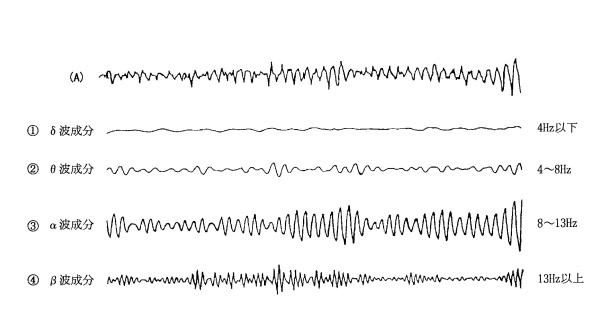
\includegraphics[width=120mm,bb=0 0 600 313]{figures/eeg.jpg}
  \caption{A. 脳波の例 1 ~ 4は周波数帯成分}
\end{figure}

\subsection{フーリエ級数展開}
さて, フーリエ変換をする目的は, 複雑すぎて解釈できない時間関数を単純な関数によって表現する事でした.\\
\\
 複雑な関数でも, 三角関数の足し合わせで表現できるという事は既に確認しましたね. 三角関数の特徴は, その振幅と角周波数が分かれば定義する事ができます. \\
角周波数とは, 1sの間にどれだけの角度波が進むかという指標で, 周波数とかから求める事が出来ます. まあ周波数って考えちゃっても大体おkです. \\
\\
 つまりフーリエ変換とは, 元関数を単純な三角関数に分け, それぞれの振幅を角周波数毎に求める事をさします.\\
\\
 このうち, 元関数f(t)を単純な三角関数の足し合わせに分解するまでをフーリエ級数展開と言い, 式では以下のようになります. 
\begin{eqnarray}
f(t) = a_0 + \sum_{\omega=1}^\infty {(a_\omega \cos(\omega t) + b_\omega \sin(\omega t))}
\label{eq:fourierkyusu}
\end{eqnarray}
式(\ref{eq:fourierkyusu})の意味はこうです. 「元関数f(t)を, 1から無限の角周波数のsin, cos波の足し合わせとして表現する」 そのまんまですね!\\
\\
ここでのaやbは変数で, 実際にはそれぞれの項毎に異なる値を取ります. 要は振幅の事ですね.\\
\subsection{複素フーリエ級数}
しかし, 式(\ref{eq:fourierkyusu})は面倒ですね. なんていったってsinとcosを分けて計算するのがだるすぎます. どうにか綺麗にできないものか...\\
\\
え?オイラーの公式を使えばいいって? ...天才かよ!!
\\
早速オイラーの公式を使って簡単にしてみましょう. 
\begin{eqnarray}
\mathrm{e}^{i\omega t} = \cos\omega t + i\sin\omega t
\label{eq:normaleuler}
\end{eqnarray}
いつもは$\pi$のところですが, 今回は空気を読んで角周波数$\omega t$に変形しています. しかし問題はあれです. オイラーの公式には愛がありますが, フーリエ級数展開の方には愛がありません. どうしたことか.\\
\\
オイラーの公式の裏を使います.
\begin{eqnarray}
\mathrm{e}^{-i\omega t} = \cos\omega t - i\sin\omega t
\label{eq:eulerminus}
\end{eqnarray}
式(\ref{eq:eulerminus})が成り立つのは大丈夫ですね?角度が実軸対称に飛んだら, cos成分は変わりませんがsin成分は符号が反転します. うちの猫でも知ってる事です.\\
\\
さて, 次に式(\ref{eq:normaleuler})と式(\ref{eq:eulerminus})を連立して解く事で式(\ref{eq:fourierkyusu})のcosとsinを置き換えます. \\
\begin{eqnarray}
f(t) = a_0 + \sum_{\omega=1}^\infty {(a_\omega \frac{\mathrm{e}^{i\omega t}+\mathrm{e}^{-i\omega t}}{2} + b_\omega \frac{\mathrm{e}^{i\omega t} - \mathrm{e}^{-i\omega t}}{2i})}
\label{eq:complexfourier}
\end{eqnarray}
この式を同類項を抜き出して整理すると
\begin{eqnarray}
f(t) = a_0 + \sum_{\omega=1}^\infty {(\frac{a_\omega - ib_\omega}{2}\mathrm{e}^{i\omega t})} + \sum_{\omega=1}^\infty {(\frac{a_\omega + ib\omega}{2}\mathrm{e}^{-i\omega t})}
\label{eq:complexfourierkai}
\end{eqnarray}
となり, 更に$\mathrm{e}^{-i\omega t}$において$\omega$を1から$\infty$まで足すのと, $\mathrm{e}^{i\omega t}$において$-\infty$から-1まで足すのは同義なため(図を書けばわかる), この3項をうまくくっつける事で
\begin{eqnarray}
f(t) = \sum_{\omega = -\infty}^\infty F_\omega \mathrm{e}^{i\omega t}
\end{eqnarray}
とおけますね!いい感じにまとまりました!!!\\
 あ, 定数部分は面倒なので$F_\omega$とおいてます. \\
\\
 フーリエ変換では, この係数たちを求めます. 
\subsection{フーリエ変換} 
 実際に式を見てみましょう.\\
\begin{eqnarray}
F(\omega) = \int_{-\infty}^{\infty} f(t)\mathrm{e}^{-i\omega t} dt
\label{eq:furier}
\end{eqnarray}

です. さっそく式(\ref{eq:furier})を解読してみましょう. 大丈夫. 基礎がしっかりできている人なら自ずと理解できるはずです.\\
\\
 まず, eの肩に $ -i\omega t $ が載っていますね. この形はどこかで見た事があります. そう, オイラーの公式ですね!!\\
 オイラーの公式にマイナスをかけたやつです. つまり $ \cos\omega t  - i\sin\omega t $ ですね. \\
式(\ref{eq:furier})は以下の式に変形できそうです.\\
\begin{eqnarray}
F(\omega) = \int_{-\infty}^{\infty} f(t)(\cos\omega t - i\sin\omega t) dt
\label{eq:furierkai}
\end{eqnarray}
 おお、結構読めてきたんじゃないですかね.\\
 分配法則が分からない輩のために, 更に式(\ref{eq:furierkai})を変形します.\\
\begin{eqnarray}
F(\omega) = \int_{-\infty}^{\infty} f(t)(\cos\omega t) - f(t)(i\sin\omega t) dt
\label{eq:furierkaikai}
\end{eqnarray}
 もう完璧ですね. ここまで解してあげれば赤ちゃんでも噛み砕けそうです!!噛み砕けない人は乳歯が生えていないのでしょう. かわいそうに...\\
\\
 さて, 式(\ref{eq:furierkaikai})を日本語にしてみましょうか.\\
 まず, 時間(t)における元関数(ここでは, ある電極で取れた脳波ですね)と, 角周波数($\omega$)のcos, sin成分それぞれとの内積を取っています. 
\\
 フーリエ変換において求めたい係数とは, 「元関数がその角周波数($\omega$)の三角関数に如何に似てるか」の指標です. そして関数の類似度の指標は内積で表せるんでしたね.一応,確認をしておきましょうか.\\
\\
Tips.\\
まずは,関数の内積を考えたときのように,イメージのしやすいベクトルで考えてみましょう.ベクトルの分解の場合には,係数を考えるのはとても簡単ですね.\\
\begin{eqnarray}
\left( \begin{array}{cc} 5\\ 3\\ \end{array} \right) = \alpha \left(\begin{array}{cc} 1\\ 0\\ \end{array} \right) + \beta \left( \begin{array}{cc} 0\\ 1\\ \end{array} \right)
\label{eq:vector}
\end{eqnarray}

はい,この時の$\alpha$と$\beta$の値を求めよ.簡単ですね.$\alpha = 5$, $\beta = 3$とすぐに解けると思います.\\
 ただまあ,こうやって感覚じゃなくて計算で求める場合には,下の式(\ref{eq:vector_right})のようにする必要があります.
\begin{eqnarray}
\alpha = \left(\begin{array}{cc} 5\\ 3\\ \end{array} \right)\left(\begin{array}{cc} 1\\ 0\\ \end{array} \right) = 5+0=5 \nonumber \\
\beta =  \left(\begin{array}{cc} 5\\ 3\\ \end{array} \right)\left(\begin{array}{cc} 0\\ 1\\ \end{array} \right) =0+3=3
\label{eq:vector_right}
\end{eqnarray}
 そう,内積です.ベクトルを直行成分に分解する際,係数を求めるには元のベクトルと分解先の「直行成分」との内積を求める訳です.\\
 これを,例によって関数に拡張します.そうすると式(\ref{eq:furier})もさらに読めるのではないでしょうか.\\
\\
 尚,面倒なので式の表記はやっぱりオイラーで表しておきます.そう,フーリエ変換の式(\ref{eq:furier})はまさに,元関数f(t)と複素指数関数との内積を計算することで,複素指数関数の係数,すなわち三角関数の大きさを産出してるわけですね!\\

次に, sin成分が負($\mathrm{e}^{-i\omega t}$)になっている理由です. 内積とは「似ている度」の指標ですね. 普通の数字やベクトルでしたら正の値になりますが, 今回のように虚数や複素数の場合は内積の結果が複素数の形をとってしまう事になります(虚数とはそういうものでしたね?).\\
\\
 それだと解釈に困ります.うざい.どうにかして虚数成分は消えた感じの結果が欲しいわけです. 虚数成分を消す...共役複素数を使えばいいですね!!!\\
\\
 実際, 自分自身との内積の正しい定義は「共役複素数をかける」です. 今までは実数で考えていたので, 気にする事はありませんでしたが複素数の場合はこの方法に則る必要があります.\\
 すなわちこうです.
\begin{eqnarray}
a = \left(\begin{array}{cc}3\\ -5i\\ 2+3i\\ \end{array} \right) \nonumber \\
(a \cdot a = )a \cdot \overline{a} = \left(\begin{array}{cc}3\\ -5i\\ 2+3i\\ \end{array} \right)\left(\begin{array}{cc}3\\ 5i\\ 2-3i \end{array} \right) = 9 + 5 + 13= 27
\label{eq:naiseki}
\end{eqnarray}
 式(\ref{eq:naiseki})の第一成分のように虚数成分を含まない場合には単純な掛け算でしたが,第二成分のように虚数成分がある場合には正負を反転させます.第三成分のような複素数の場合は虚数成分だけ反転です.\\
\\
 つまり,今までやってた内積の計算方法はたまたま虚数成分がないからそのままかけてただけで,一般的な定義はこちらということですね.
\\
 これにより, ある角周波数成分 $\mathrm{e}^{i\omega t}$と元関数f(t)の内積を求める際に$\mathrm{e}^{-i\omega t}$を用いるわけです. まあ, やってるのは普通に内積です.\\
\\
\\
 内積とは, 「どれだけ似ているか」の指標でしたね. つまりここで, 元関数は角周波数($\omega$)の三角関数とどれだけ似ているかを見ているわけです!!\\\\
 そしてその結果を $-\infty$ から$\infty$ までの範囲で積分 ... 足し算しています.\\\\
 この値がF($\omega$)らしいですね. さて, こいつはどういった条件でどういった値を取るかというと, 元関数の中に角周波数($\omega$)の成分が多ければ多い程, 内積の値は1に近くなります. \\
 という事はその総和も大きくなります. 逆に値が小さいという事は内積の値も小さい ... つまり元関数の中に角周波数($\omega$)の成分は少ないという事になりますね!!\\
\\
 こうして, 複雑怪奇な時間関数を周波数関数に変換(というか見方を変える)事によって, より解釈のしやすい形に変換するのがフーリエ変換の強みです.\\
\\
 実際にはF(ω)のうち, 「$x_1Hz$は成分が大きくて, $x_2Hz$は成分が小さいね」といった事が分かるようになるわけです.
\subsection{フーリエ変換の実用}
 実際には, 式(\ref{eq:furier})によって無限の周波数成分を抜き出し, それぞれの振幅を求める事で, 元関数(t)はそれぞれの周波数をそれぞれの振幅倍したsin波の足し合わせで出来てるね!と解釈します.\\\\
 例えば, 「タスク1をやらせた時の被験者君は5 -- 7Hzくらいの脳波がよくでているね!」「タスク2の時には大して強くないね。てことはタスク1と5 --7Hzの脳波には何か関係がありそうだね!!」といった具合です. 論文にもそのまんま書かれています.
\\\\
 人はこれを周波数分解といい, これを使った解析が周波数解析だとかスペクトル解析と呼ばれる種々の解析になります!!(上の「」に入ってるのも周波数解析による解釈)
\section{wavelet 変換}
\subsection{フーリエ変換の弱点と定常性}
万能に思えるフーリエ変換ですが, 実は弱点があります.結論から言うなれば,それは「元関数f(x)に定常性を仮定してしまっている」です.関数の定常性とは,平均や自己共分散が時間に陽に依存していない,同じ時点数ならどこで切っても同じ形になってる,などといった特徴を指します.簡単に言えば,どれだけ時間が経っても同じ関数の形を保っているということです.以下が(強い)定常性を満たす関数の例です.
\begin{eqnarray}
y = 3\\
y = sinx
\end{eqnarray}
 そりゃそう,ですね.どちらも先の定義を満たしているのがわかるかと思います.三角関数は周期性を持った関数なので,当然定常性を満たすことになります.\\ \\
 さて,ここで問題なのがフーリエ変換の方針です.「すべての関数は,無限の複素サイン波の足し合わせで表現することができる」でしたが,これはより正確には「すべての(定常性をもつ)関数は〜」です.\\ \\
 何故なら,周期関数であるサイン波との積は,仮に元関数が同様に周期性を持つ,定常性をもつ関数でない場合にはどのタイミングで内積を求めるかによって値が変わってしまいます.\\
\\ 
 これはとても困る.\\
 元関数の性質を,内積によって圧縮しているのにどのタイミングで計算するかによって値が変わるんじゃ話になりませんよね.\\
\\
 なのでフーリエ変換をする際には,元関数f(t)に定常性を仮定する必要があります.時間に陽に依存した関数ではない,とすることです.\\
\\
 逆に言うと,定常性を満たさない関数に対しフーリエ変換は使えません.計算が出来ない訳じゃないけど,正しい分析をすることが出来ません.役立たずです.\\
\\
\\
 勘の良い読者諸君ならお気づきだろうが(物理の本でよく見るコレ,一度言ってみたかった),これでは脳波の解析に使えなさそうじゃないですか?使えないですよね?\\
\\
 え?なんでそうなるのって?え,なに,お前の脳波は飯食ってる時もデートしてる時も数学やってる時もずっと同じなん?\\ \\
 きっしょ.\\
\\
 普通,脳波はずっと同じなんてことはないですよね.脳が体を操作したり感覚の処理を行なっているとする我々の立場が本当に正しいのであれば,脳という処理系は入力の値によってその振る舞いを変えるし,同様に出力を出すためにも振る舞いを変えるはずです,\\
\\
 そう,脳波は定常性を持っていないのです.困った.フーリエ変換は使えないじゃないか.なんのために苦労してフーリエ変換やったと思ってるんだ馬鹿野郎.時間返せ.\\
\\
\subsection{窓付き,短時間フーリエ変換}
しかし,逆に考えるとそもそもそんなガチな定常性を持った関数の方が自然には少ないだろうし,そもそも無限時間の積分とかできる訳ないだろって感じだし,そのまんまのフーリエ変換が厳しすぎるだけな気もします.どうにかもう少し現実的な妥協案を考えましょう.ということで考案されたのが,窓付フーリエ変換だとか短時間フーリエ変換だとか言うやつらです.\\
\\
 ざっくりと説明しましょう.やつらの用意した言い訳はこうです.\\
「確かに無限時間なら定常性がないけど,短い時間の中では?その中では定常性を持ってるぽく振る舞うことは十分にあるよね?」\\
 うーん,たしかに?厳密さにかけるし,”短い時間”ってどれくらいよって感じだし,それでもダメっぽい可能性もあるっしょだったり,色々と文句はありますが,まあこう言うことです.\\
\\
 ということで,元関数f(t)をぶつ切りにしていきます.ただここで問題です.ただただ元関数を切り取るだけで良いのかというとそうではありません.だって連続的な値をとる波なのに無理やり途中で切られたら,断面が変な形になってしまいますよね.とても不自然だし,これだと超高周波成分なのかな?みたいに解釈されてしまいます.\\
\\
 それは困る.脳波の場合,周波数成分を見るといつも高周波が乗ってるね!高周波が大事なんだ!みたいな誤った解釈につながってしまいます.\\
\\
 そこで,どうにか切り取った「窓」の両脇の影響は減衰させていく必要が出てきます.どうするか.影響を減らすためには,単純に端に行くにつれて波を小さくしていけばいいですね.窓の真ん中が一番影響が乗り,端に行くほど影響が小さくなる,いわゆる山形の信号に整形してやれば良い訳です!!\\
\\
\\
 山形に窓を整形するために,元信号にかけるフィルタのような働きをする関数を,窓関数と言います.よく用いられるのはガウス関数です(\ref{eq:normal}).形綺麗だしね.というわけで,窓付きフーリエ変換の式は以下のようになります.

\begin{eqnarray}
STFT_{f,w}(t, \omega) =X(\omega)= \int_{-\infty}^{\infty} f(\tau)w(\tau - t)\mathrm{e}^{-i\omega t} d\tau
\label{eq:stft}
\end{eqnarray}

ここでf(t)は元関数,w(t)は窓関数であり,元関数と窓関数で畳み込みを行なっているわけですね!畳み込み!Basicの方で勉強しといてよかったですね!\\
 んで,よく使われる窓関数はガウス関数である.ガウス関数を窓関数として使う場合はこんな感じ(式\ref{eq:stft_gauss})になるのかな?

\begin{eqnarray}
STFT_{f,w}(t, \omega) = X(\omega) = \int_{-\infty}^{\infty} f(t) \frac{1}{\sqrt{2\pi\sigma^2}}e^{-\frac{t^2}{2\sigma^2}}\mathrm{e}^{-i\omega t} dt
\label{eq:stft_gauss}
\end{eqnarray}

整理すると,短時間フーリエ変換は元信号に窓関数をかけて整形したデータをフーリエ変換にかける事でした.\\
\\
 がしかし,これでもまだ,というか新しい問題が発生してしまいます.その問題を解決するために開発されたのが,いよいよ本題であるウェーブレット変換です. 
\subsection{不確定性原理}
さて,短時間フーリエ変換の何が問題になっているのかというと,元信号に窓関数をかけてしまっている事です.これにより,どの周波数帯域のデータを見るにしても同じ時間窓を利用する事になっているので,時間窓長は一定で,カーネル(複素サイン)の角周波数$\omega$を変数とする事になります.\\
\\
 大丈夫?わかる?
\\
 ここで問題になるのが,周波数分解能と時間分解能のトレードオフ,不確定性原理です.\\
\\
 つまり,高周波になるほど時間分解能が上がり周波数分解能が下がる,低周波になるほど時間分解能が下がり周波数分解能が上がる,という現象です.\\
\\
 ちょっと想像すればわかります.人間の脳も同じですから.1Hzの振動と2Hzの振動を区別するのは容易ですよね?1秒に1回殴られるのと1秒に2回殴られるのは大きく違います.これが周波数分解能が高い状態です!\\\\
 でもお前らみたいな陰キャはやっぱいじめられっ子なので,殴られる回数もそんなもんじゃないでしょう.きっと秒間100発とか殴られてるはずです.かわいそうに.そんなお前らにとっては,秒間100発殴られるのも101発殴られるのも変わらないよね(笑).これが周波数分解能が低い状態.\\
\\
 時間分解能については,時間をどれだけ区切って考えられるかなので高周波ほど高いのは自明ですね.\\
\\
 さて,分解能について理解したところで短時間フーリエに戻りましょう.先ほど確認したように,短時間フーリエでは「元関数に窓関数をかけて,それを変数$\omega$のフーリエ変換にかける」訳でしたね?\\
\\
 こうすると,どんな周波数でも窓の長さは一定です.もうわかったね?\\
\\
 そう,短時間フーリエでは低周波と高周波でそれぞれ時間と周波数の分解能の良し悪しが反転してしまっているのです.低周波ほど信号のタイミングが掴みにくくなるし,高周波ほど周波数の違いが分からなくなってくる.困る.同じスケールで議論ができないのはクソです.

\begin{figure}[H]
\label{im:furiers}
  \centering
  \includegraphics[width=100mm,bb=0 0 600 300]{figures/furiers.png}
  \caption{短時間フーリエのイメージ.周波数によって窓の長さが違う=波の数も違う}
\end{figure}


\subsection{Wavelet変換}
 この問題を解決するためにはどうするか.簡単ですね.周波数に依存して窓の長さが変えられるようになれば良い訳です.つまり高周波を見たい時にはカーネルが短く,低周波を見たい時には長くなればいいわけです.\\

\begin{figure}[H]
\label{im:wavelets}
  \centering
  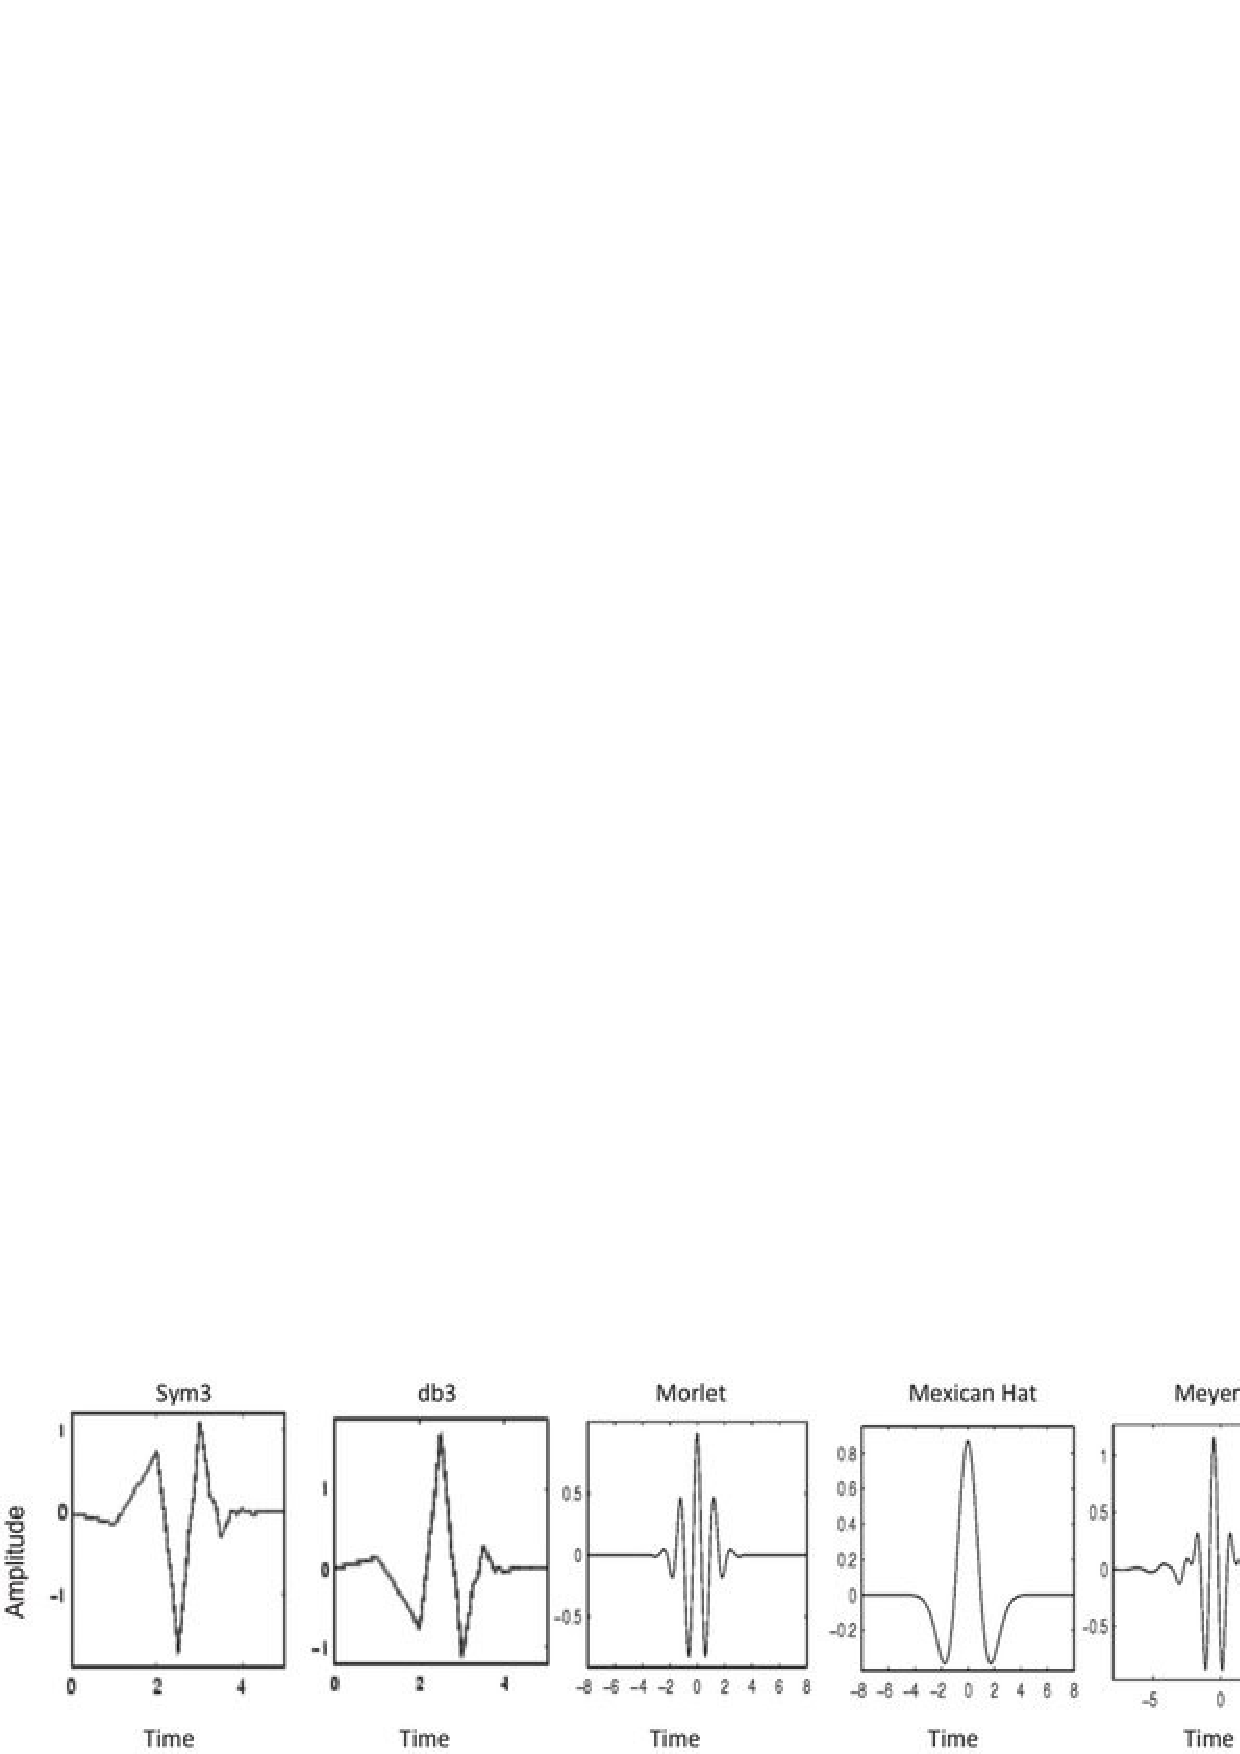
\includegraphics[width=100mm,bb=0 0 600 300]{figures/wavelets.png}
  \caption{waveletのイメージ.周波数によって窓の長さが違う,波の数は同じ}
\end{figure}

こうすると(どうやるのかはさておき),周波数によって窓の長さが違うので,いれられる波の数も同じ=時間分解能や周波数分解能が同じ(っぽい)ように計算ができます.これがWavelet変換のモチベです.\\
\\
 基本的な方針はフーリエと変わらず,元関数とカーネルとの内積によって周波数成分を抜き出す積分変換です.ウェーブレット変換の基本形は以下です.\\

\begin{eqnarray}
W_\psi[f(t)]  = T(a,b) = \int_{-\infty}^{\infty} f(t)\psi_{a,b}(t) dt
\label{eq:wavelet_transform}
\end{eqnarray}

ここで用いるカーネル$\psi_{a,b}(t)$が(マザー)ウェーブレットです.フーリエ変換の時は複素サインでしたね.ウェーブレット変換とは,カーネルにウェーブレットを利用する事によって不確定性原理の壁を乗り越えようというものです.\\
\\
 そのウェーブレット変換ですが,カーネルに用いる関数の事をマザーウェーブレットと言います.そんなマザーウェーブレット$\psi$を,良い感じに調整して作るのがウェーブレットです.式(\ref{eq:wavelet})はマザーウェーブレット$\psi$からウェーブレットを作る公式.

\begin{eqnarray}
\psi_{a,b}(t)  = \frac{1}{\sqrt{a}}\psi(\frac{t-b}{a})
\label{eq:wavelet}
\end{eqnarray}

aとbが変数で,こいつらを変調させていく事でいろんなウェーブレットを作成し,そいつと元関数との内積を見ていくのがウェーブレット変換です.この変数について考えていきましょうか.\\
\\
 まず簡単なのはbの方ですね,時間tを調整している訳だから,単純にウェーブレットの位置を動かしてくれます.シフトと言います.つまり元関数のうちどの時間について変換をするかという事です.高校数学で二次関数のグラフを横移動させたときのアレに似てます.\\
\\
 次はaです.スケールと言います.aの値を変える事で,窓の幅が変わります.割り算してるしね.aが大きいほど窓は広く,aが小さいほど狭くなります.$\sqrt{a}$はスケーリングに対して,つまり窓幅に対してエネルギーが一定になるように調整しているだけ.本質は分数のとこにあります.\\
\\
 さて,ここで勘の良い読者ならお気づきでしょう.マザーウェーブレットを変形させて作るのがウェーブレットという事でした.そう.つまりウェーブレット変換における変数はスケールとシフトのa,bなのです!!\\
\\
 フーリエ変換の変数は角周波数$\omega$でしたが,ウェーブレットにおいてはスケールとシフトなのです.もっというと,周波数$\omega$は定数として扱われます.つまり色んな周波数に対して内積を見ていくのではないという事.この点がウェーブレットが不確定性原理に打ち勝てる秘訣です.\\
\\
 問題は,そうするとどうやって周波数の区別をするんだという事になります.そこで先ほどの変数a(スケール)の存在意義がわかってきます.図(\ref{im:wavelets})から見て取れるように,窓の長さを変える事によって中の波の周波数も変わっています.これによって周波数の差を表現しているわけですね!!\\
\\
短時間フーリエ変換とは,時間窓長を固定し角周波数を変える積分変換.\\
ウェーブレット変換とは,各周波数を固定し時間窓長(全体スケール)を変える積分変換.\\
\\
というわけですね!!違いが分かったでしょうか!!\\

\subsection{Morlet Wavelet}
さて,ウェーブレット変換の概要をつかめたところで,実際に用いられるマザーウェーブレットについて考えていきます.色んな奴がいますが,ここでは脳波解析でよく使われている Morlet Waveletについて解説します.\\
\\
 こいつは非常に単純.今の皆さんならすぐにわかるはずです.なんていったって複素サインにガウスをかけた奴ですから.式は以下(\ref{eq:morlet_wavelet})です.

\begin{eqnarray}
\psi(t) = \frac{1}{\sqrt{2\pi\sigma^2}}e^{-\frac{t^2}{2\sigma^2}}\mathrm{e}^{-i\omega_0 t} dt
\label{eq:morlet_wavelet}
\end{eqnarray}

ね?\\
 もうみんななら分かるはず.ガウス窓付き短時間フーリエと同じノリです.これを使ったウェーブレット変換が以下(\ref{eq:morlet_wavelet_trans})になります.

\begin{eqnarray}
T(a,b) =  \int_{-\infty}^{\infty} f(t) \frac{1}{\sqrt{2\pi\sigma^2}}e^{-\frac{(\frac{t-b}{a})^2}{2\sigma^2}}\mathrm{e}^{-i\omega_0 (\frac{t-b}{a})} dt
\label{eq:morlet_wavelet_trans}
\end{eqnarray}

ほとんどガウス窓付き短時間フーリエと同じですね!並べてみましょう.
\\\\
 短時間フーリエ変換.
\begin{eqnarray}
STFT_{f,w}(t, \omega) = X(\omega) = \int_{-\infty}^{\infty} f(t) \frac{1}{\sqrt{2\pi\sigma^2}}e^{-\frac{t^2}{2\sigma^2}}\mathrm{e}^{-i\omega t} dt
\end{eqnarray}


Morlet Wavelet変換.


\begin{eqnarray}
W_\psi[f(t)] = T(a,b) =  \int_{-\infty}^{\infty} f(t) \frac{1}{\sqrt{2\pi\sigma^2}}e^{-\frac{(\frac{t-b}{a})^2}{2\sigma^2}}\mathrm{e}^{-i\omega_0 (\frac{t-b}{a})} dt
\end{eqnarray}

とても似ていますね.\\
 ちがっているのは,短時間フーリエは時間(窓長)を固定していて変数$\omega$の関数として記述されるのに対し,ウェーブレット変換は周波数を表す$\omega$は定数$\omega_0$で固定されスケールがaとbの変数によって調整されるaとbの関数として記述されている点です!!\\
\\
 他にも,ガウス窓付き短時間フーリエの方は元信号にガウスをかけてから複素サインと内積を取ってる一方でMorlet Waveletは複素サインにガウスをかけてから元信号との内積を取っているなどといった違いもあります.

\section{時間周波数解析の解釈}
フーリエやウェーブレットの結果から,power,frequency,phaseをとりだす方法について書くぞい







\chapter{統計処理}
応用に入れるべきか基礎にいれるべきか悩みましたが, 文量がかなりのものになるため応用に入れる事にしました. 統計処理とは, 実際に実験やアンケートを通して集めたデータを解釈する際に必要になる処理です. 論文を読むためにも必須, というか一番大事な項目なので頑張りましょう.
\section{確率分布}
\subsection{確率分布と確率密度関数}
確率とは, 起こりうる全体の事象のうち, ある事象がどれくらいの割合で起こるのかを表します. 確率分布とは, 起こりうる事象それぞれの確率がどのような分布をしているかです. \\
確率分布関数とは, 実際に確率分布をプロット(横軸に事象, 縦軸に確率)した際に現れる分布の形を表現する関数の事です. 場合によっては事象は離散分布になる事もあるため, その場合は密度関数は定義できないか, あるいは離散値を疑似的に連続値に見立てる事で定義されます. イメージとしては折れ線グラフを作る時のあれです. 各事象の度数を表す点を結んでく感じ.\\

\subsection{一様分布/ベルヌーイ分布/2項分布/ポアソン分布}
まずは簡単な分布から見て, 徐々に複雑なものを見ていきます. 今回は脳の数学であまり使わない気がするやつらはまとめて雑に確認します.\\
\subsubsection{一様分布}
例えばサイコロを振った時に出る目の確立分布を考えると, 当然6つの事象それぞれがすべて$\frac{1}{6}$で表せるため, 確率分布をプロットすると以下のようになります.\\
\begin{figure}[H]
\label{im:uniform}
  \centering
  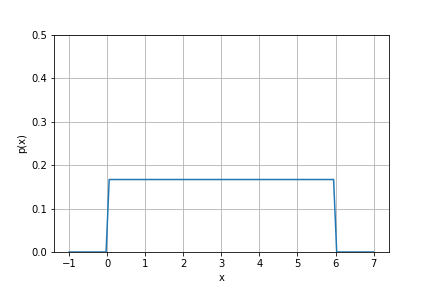
\includegraphics[width=120mm,bb=0 0 432 288]{figures/uniform.png}
  \caption{サイコロの確立分布(一様分布)}
\end{figure}

一様分布は確率密度関数を定義するまでもないのですが, 勉強のためにあえてやるとすると以下のようになります.

\begin{eqnarray}
\label{eq:uniform}
f(x) = \frac{1}{6} (0 \leq X \leq 6)
\end{eqnarray}

定義域が0から6で, いずれの点においても$\frac{1}{6}$の確立で目がでるよってことですね. 簡単です. また確率を考える際, 式(\ref{eq:uniform})のように左辺の(x)と右辺定義域内にいる(X)で使い分けがなされます. Xは確率変数を表し, 実際の値は取りません. 観測されて確定した時にはxとして表現されます. 今回のXとxの関係は

\begin{eqnarray}
X = [x_1, x_2, x_3, x_4, x_5, x_6]
\end{eqnarray}
のような感じです. \\
\\
平均E(X)及び分散V(X)は

\begin{eqnarray}
E(X) = \frac{a+b}{2}\\
V(X) = \frac{(b-a)^2}{12}
\end{eqnarray}

です. 興味ないので証明とかやりません. 僕も知らない.
\subsubsection{ベルヌーイ分布}
ベルヌーイ分布は, 1か0かです. ある事が起きるか起きないか, 成功するかしないかなどの2値分類ですね. 超簡単です!!\\

\begin{figure}[H]
\label{im:bernoulli}
  \centering
  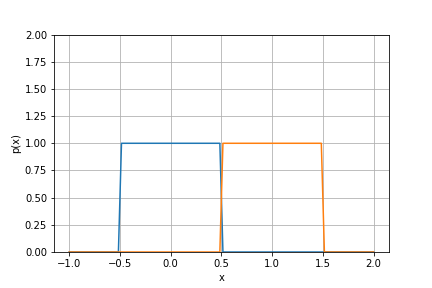
\includegraphics[width=120mm,bb=0 0 432 288]{figures/bernoulli.png}
  \caption{ベルヌーイ分布}
\end{figure}
今回は1:1の図になっていますが, もちろん1:5くらいの割合になる事もあります. たとえばサイコロで1が出るか出ないかとか. 以上.\\
\\
関数はこんな感じかな
\begin{eqnarray}
f(x)=
  \left\{
    \begin{array}{l}
      p \qquad \qquad \qquad (x = 1) \\
      q(=1-p)  \qquad (x=0)
    \end{array}
  \right.
\end{eqnarray}

平均E(X)及び分散V(X)は

\begin{eqnarray}
E(X) = p\\
V(X) = pq
\end{eqnarray}

です. 興味ないので証明とかやりません. 僕も知らない.
\subsubsection{2項分布}
2項分布は「同じことを何回も繰り返した時, ある事柄が何回おこるか」の確立分布です. こいつは式を見れば早いですね.

\begin{eqnarray}
\label{eq:binomial}
f(x) = {}_n\mathrm{C}_x p^x(1-p)^{n-x}
\end{eqnarray}

式(\ref{eq:binomial})の右辺左側にある${}_n\mathrm{C}_x p^x$は, 確率pで起こる事象Aが, 全体nのうちx回でたという意味で, 右側の$(1-p)^{n-x}$は確率(1-p)で, Aが起きなかった回数が(n-x)回出たという意味です.\\
これらを掛け合わせているので, 何回当たって何回外れたかを表す式ですね.

\begin{figure}[H]
\label{im:bernoulli}
  \centering
  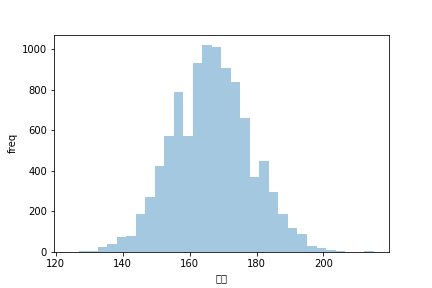
\includegraphics[width=120mm,bb=0 0 432 288]{figures/binomial.png}
  \caption{ベルヌーイ分布}
\end{figure}

平均E(X)及び分散V(X)は

\begin{eqnarray}
E(X) = np\\
V(X) = np(1-p)
\end{eqnarray}

です. 興味ないので証明とかやりません. 僕も知らない.

\subsubsection{ポアソン分布}
ポアソン分布は「稀な事象が一定時間内にどれくらい起きるか」です.\\
たとえば, ある月にある地域で起きた交通死亡事故の件数とかです. 修羅の国やグンマ―, あるいは名古屋でもない限り, 普通は0か多くて2件とかですよね.\\
\\
確率密度関数は以下です.
\begin{eqnarray}
f(x) = \frac{\lambda^x}{x!}e^{-\lambda}
\end{eqnarray}

平均E(X)及び分散V(X)は

\begin{eqnarray}
E(X) = \lambda\\
V(X) = \lambda
\end{eqnarray}

です. こいつの場合, 平均も分散も同じ定数$\lambda$なので, こいつの値だけで形が決まります. $\lambda$がどんな値なのか, どうやって決まるのかは知りません. 使う事があれば足します.\\

\begin{figure}[H]
\label{im:poisson}
  \centering
  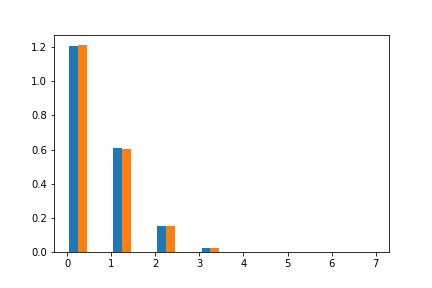
\includegraphics[width=120mm,bb=0 0 432 288]{figures/poisson.png}
  \caption{ポアソン分布}
\end{figure}

\subsection{正規分布}
\subsubsection{正規分布とは}
さて本題です. 数ある確率分布の中でも抜きんでて重要な分布, 正規分布, またの名をガウス分布です. 世の中の多くの事象がこの分布に従っていて, また従っていると仮定して統計的処理がされています. 今後の統計学の基礎になるのでしっかり理解しましょう.\\
\\
正規分布は, 平均E(X)が母集団の平均μと等しく, 分散V(X)も母集団の分散$\sigma ^2$と等しくなる分布で, 確率密度関数は以下になります.

\begin{eqnarray}
\label{eq:normal}
f(x) = \frac{1}{\sqrt{2\pi\sigma^2}}e^{-\frac{(x-\mu)^2}{2\sigma^2}}
\end{eqnarray}

いや, うん. 分かる. やべえよな. ただまぁ, なんでこんな殺意高めな式になるのかは正規分布のグラフを見れば理解できます. 母集団の平均が50, 標準偏差20の正規分布だとこうなります.

\begin{figure}[H]
\label{im:normal}
  \centering
  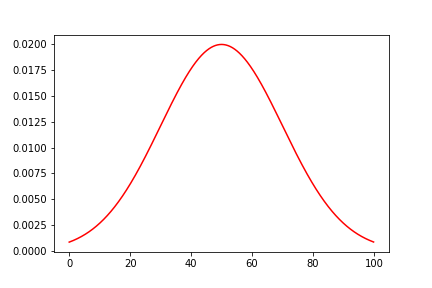
\includegraphics[width=120mm,bb=0 0 432 288]{figures/normal.png}
  \caption{正規分布}
\end{figure}

定義通り, 確率変数の平均も50, 分散も400(20の二乗)になっていますね!!これが正規分布です. 綺麗ですね.\\
\\
\subsubsection{確率密度関数の導出}
さて, 式(\ref{eq:normal})の解説です. まずややこしいとこを全て消し飛ばし, 以下のように変形しましょう. 

\begin{eqnarray}
\label{eq:normal2}
f(x) = e^{-x^2}
\end{eqnarray}

\begin{figure}[H]
\label{im:normal}
  \centering
  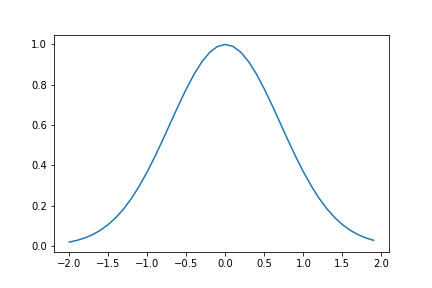
\includegraphics[width=120mm,bb=0 0 432 288]{figures/normal2.png}
  \caption{式(\ref{eq:normal2})の図}
\end{figure}

この関数の説明はいりませんね? 指数関数の二乗の負版です.\\
まず, 世の中の多くの事象は平均値を取る確率が一番大きく, 平均値から離れるにつれその値を取る確率は小さくなることが知られています. んで, これをどう数式で表現すれば良いかと悩んだ末考えだされたのが正規分布関数だと思ってください.\\
そうすると, とりあえず釣り鐘型の関数が欲しいという事で式(\ref{eq:normal2})を考えました. 実際これでほぼ完成です.\\
ただ, これは任意定数がないため平均が0, 分散(幅)も一定ですね. これでは実用できません. そこで任意定数を導入し, 平均値と分散を可変にします. 平均値, つまりこのグラフの頂点の位置を動かすのは簡単ですね?\\

\begin{eqnarray}
\label{eq:normal3}
f(x) = e^{-(x-\mu)^2}
\end{eqnarray}

です. 高校数学でやりましたね.\\
\\
次に, 分散...つまりこの釣り鐘の幅というか広がり方を変えます. \\

\begin{eqnarray}
\label{eq:normal4}
f(x) = e^{-\frac{(x-\mu)^2}{\sigma^2}}
\end{eqnarray}

平均に比べて一寸難解かもしれません. σ, つまり標準偏差で割る事で, σの値が小さければ鋭く, 大きければ扁平なグラフになりますね?\\
\\
ただ, σは正負が定まらないため, 二乗して分散の形にする事で符号を一定にするわけです. \\
\\
ともあれ ... これで, 母平均と母分散によって形を変える釣り鐘型分布が完成です!!めでたい!!\\

\begin{figure}[H]
\label{im:normal}
  \centering
  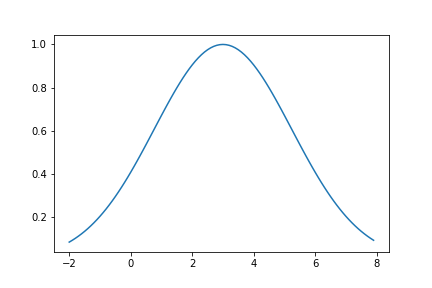
\includegraphics[width=120mm,bb=0 0 432 288]{figures/normal4.png}
  \caption{式(\ref{eq:normal4})の図.(平均3, 分散10の場合)}
\end{figure}

え?式(\ref{eq:normal})と違うじゃないかって?\\
せっかちだなぁ......余裕がない人間はモテないぜ?\\
\\
ん?僕ですか?別に同期や後輩が軒並み揃って国内/国際学会に行ってたり,  ペーパーがアクセプトされてたりするからって全然焦ってないですよ?もう余裕すぎてこんな同人誌書いてるくらいですもん. \\
\\
うん. これ書いたら暫く更新やめます.
\\
\\
まあ, グラフの形は実際これで完成なのです. ただ, 今我々が求めていたのは正規分布の「確率密度関数」でしたね?\\
\\
確率の密度なのですから, 当然合計して1にならないといけないわけで, 先程の式(\ref{eq:normal4})ではその点がダメなのです. ちゃんと全確率点での値を足して1になるように正規化する必要があります.\\
\\
つーわけで積分方程式を解きましょ...っとその前に, 出てくる計算結果を綺麗にするために式(\ref{eq:normal4})に細工をし, $\sigma^2$を$2\sigma^2$にしておきます. 2が付きましたが, グラフの性質自体は変わりませんね?\\
\\
では積分方程式.
\begin{eqnarray}
\int_{-\infty}^{\infty} c e^{-\frac{(x-\mu)^2}{2\sigma^2}} dx= 1
\end{eqnarray}
を解きます...出来たものがこちらです.

\begin{eqnarray}
\label{eq:c}
c = \frac{1}{\sqrt{2\pi\sigma^2}}
\end{eqnarray}

式(\ref{eq:c})で得られたcを改めて式(\ref{eq:normal4}の変形版)に代入すると

\begin{eqnarray}
f(x) = \frac{1}{\sqrt{2\pi\sigma^2}}e^{-\frac{(x-\mu)^2}{2\sigma^2}}
\end{eqnarray}

が出てきましたね!良かった良かった. 以上が正規分布の確率密度関数の導出工程でした. フーリエなんかに比べれば雑魚ですね!ワンパンでした!\\

\subsubsection{100p\%点}
次. 正規分布を学ぶ意味は, この概念があるからといっても過言じゃない重要な性質です. 正規分布は平均が丁度真ん中で, 広がり方は分散によって定義される左右対称な特殊な分布でしたね?\\\\
つまり, 平均周辺程高確率で観測され, 裾野ほど「レア」な事象というわけです.\\\\
この性質を利用して, 正規分布には「100p\%点」と呼ばれる指標を導入する事が出来ます. これは「その点以上(以下)の部分の確率の合計がpになる境界」を指します. x軸の正方向なら上側, 負方向なら下側, 両方を指すなら両側100p\%点です. \\\\
言葉だとややこしいですが, グラフで見れば一瞬で分かります.


\begin{figure}[H]
\label{im:upper}
  \centering
  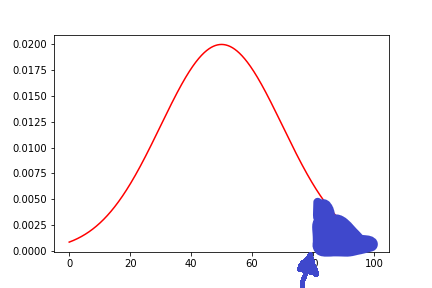
\includegraphics[width=120mm,bb=0 0 432 288]{figures/upper_p.png}
  \caption{正規分布の上側5\%点}
\end{figure}

\begin{figure}[H]
\label{im:bilateral}
  \centering
  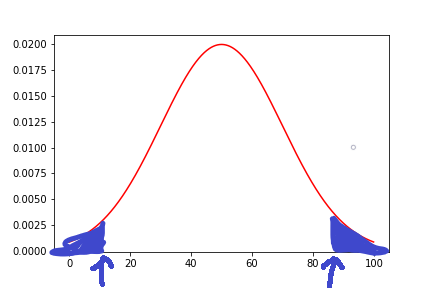
\includegraphics[width=120mm,bb=0 0 432 288]{figures/bilateral_p.png}
  \caption{正規分布の両側5\%点}
\end{figure}

上側5\%に比べ, 両側5\%は左右に領域が分散した分上側の領域が狭くなってるのに注意です. \\
\\
だいたい, 正規分布でよく用いられるのは上下両側の5\%と1\%点です. 何に使うのかはあとで説明するので, ひとまず概念だけ覚えておいてください.

\subsection{t分布}
少ない標本数をもとに母分散がわかっていない母集団の母平均推定に使われるのがt分布です. 詳しくは推定の項で触れるので, ここでは確率密度関数と性質の確認をします.

\begin{eqnarray}
\label{eq:student}
f(x) = k(1 + \frac{x^2}{\alpha})^{-\frac{\alpha+1}{2}}
\end{eqnarray}

式(\ref{eq:student})がt分布の確率密度関数です. ここでkは定数, αは自由度という指標で, この形を「自由度αのt分布」と表現します. 自由度とは何かはここでは説明しませんが, 母集団によって算出できる値です. それ以外の部分では正規分布に似ていますね. 実際, 自由度αが十分に大きい場合には正規分布になります. ただこいつの平均と分散は

\begin{eqnarray}
E(X) = 0\\
V(X) = \frac{\alpha}{\alpha-2}
\end{eqnarray}
です. 

\begin{figure}[H]
\label{im:student}
  \centering
  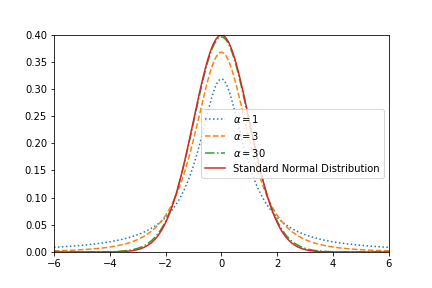
\includegraphics[width=120mm,bb=0 0 432 288]{figures/student.png}
  \caption{自由度の異なるt分布と標準正規分布}
\end{figure}
自由度の異なるt分布と標準正規分布の比較です. 標準正規分布とは, 正規分布のうち平均が0, 分散が1のやつです. αの値が大きいとほぼ同じ形になる事が分かると思います.\\
\\
では何に使うのかですが, そこはひとまず置いておきます. とにかくこういう分布があるのです.


\subsection{F分布}
F分布は, 少し特殊な形をしていますが非常に重要です. どう重要かというとF分布はこれまでの分布と異なり, 2つの母集団から得られた標本分散の比の確率分布になります. これの何がすごいのかというと, 例えば図(\ref{im:f_dist})は自由度が3の母集団Aと自由度が10の母集団BのF分布ですが, 「普通は」この組み合わせだと0から2あたりの値になる事が多いのです. \\
\\
しかしもし今, 自由度3と10のとある母集団A,B間でF値を取ったら6とかが出たとします. \\
通常はありえない値, つまり統計的に考えると「自由度だけでなく分散そのものに差がある = A,Bの母集団は異なる」となるわけですね. こちらも詳しくは後程. 式はえぐえぐです. 震えろ.

\begin{eqnarray}
f(x) = \frac{kx^{\frac{m}{2}-1}}{\{1 + (\frac{m}{n})x\}^{\frac{m+n}{2}}}
\end{eqnarray}

こいつの導出はいいです. 僕もわからん. 気が向いたら勉強してまとめるかも. 例によってkは定数, m,nは標本集団2つのそれぞれの自由度です. こいつは「自由度m,nのF分布」と表現されます. 今はそれだけ. 続いてグラフです. 幸いこっちは簡単.

\begin{figure}[H]
\label{im:f_dist}
  \centering
  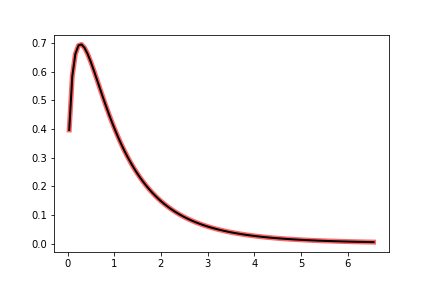
\includegraphics[width=120mm,bb=0 0 432 288]{figures/f_dist.png}
  \caption{自由度3.10のF分布}
\end{figure}

恒例の平均値と分散です. こいつらも殺意高めだけど覚える必要は今のところ皆無だと思ってます.

\begin{eqnarray}
E(X) = \frac{n}{n-2}\\
V(X) = \frac{2n^2 (m+n-2)}{m(n-2)^2(n-4)}
\end{eqnarray}

\subsection{$\chi^2$分布}
ラスト. $\chi^2$分布です. こいつも重要です. 我々は結果を理論に落とし込む時, なんらかの数式に近似したり回帰したりするわけですが, 実際問題理論と観測値が完全に一致するなんていう事はまれで, 様々な要因で若干の誤差が生じます. その誤差が「誤差」なのか「理論の誤り」なのかを評価する時に使うのがこの分布とそれに基づく検定です. \\
\\
式はこちらです. 
\begin{eqnarray}
f(x) = k\chi^{\frac{\alpha}{2}-1}e^{-\frac{\chi}{2}}
\end{eqnarray}

またえぐえぐですね. えぐえぐと言えば, 筆者は声優の江口拓也さんが「やはり俺の青春ラブコメは間違っている」のラジオでやっていた「ぼっちラジオ」が大好きです. どうせこんな数学の同人誌読んでる人は陰キャだし, 楽しめると思います. 是非YouTubeで検索してみてください.\\
\\
さて, 例によってここのαは自由度, kは定数です.\\
幸い, どこの説明を見てもこの式は使わないと言われているので覚えなくていいでしょう.\\
\\
平均値と分散です.
\begin{eqnarray}
E(X) = \alpha \\
V(X) = 2\alpha
\end{eqnarray}
簡単すぎワロタww\\
ついでグラフです.


\begin{figure}[H]
\label{im:chi}
  \centering
  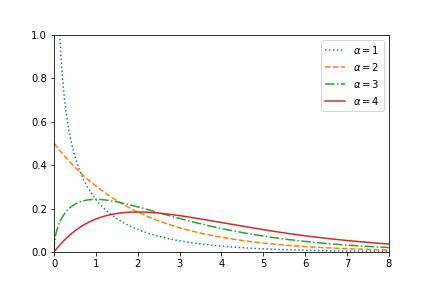
\includegraphics[width=120mm,bb=0 0 432 288]{figures/kai.png}
  \caption{自由度の異なる$\chi^2$分布}
\end{figure}
 こいつは結構F分布に似てますね. ただ注意が必要なのは, F分布は標本分散の比に関する分布ですが$\chi^2$分布は標本分散そのものの分布です.

\section{統計的推定}

\subsection{サンプリングとは}
\subsection{中心極限定理}
\subsection{普遍分散}
\subsection{点推定}
\subsection{区間推定}
\subsubsection{信頼度/信頼区間/100p\%点}

\section{統計的検定}
\subsection{仮説検定と有意差}
\subsection{母平均の変化の検定}
\subsubsection{母分散既知}
\subsubsection{母分散未知}
\subsubsection{十分に大きい標本の場合}
\subsection{母比率の変化の検定}
\subsection{母平均の違いの検定}
\subsection{母分散の違いの検定}
\subsection{母比率の違いの検定}
\subsection{第一種/第二種の過誤}

\section{分散分析}
\subsection{分散分析とは}
\subsubsection{因子と水準}
\subsubsection{n元配置の分散分析}
\subsubsection{分散分析の繰り返し}
\subsection{一元配置の分散分析}
\subsection{二元配置の分散分析}
\subsection{繰り返しのある二元配置の分散分析}
\section{回帰分析}
\end{document}